\chapter{Results}
\label{ch:results}

\section{Fiducial \WZjj cross section measurement}

The cross section for \WZjj production, without separating by production mechanism,
is measured with a combined maximum likelihood fit to the 
observed event yields by leptonic decay channel of the $\PW$ and $\PZ$ bosons as 
described in Section~\ref{sec:statistics}.
A signal strength $\mu_{\WZjj}$, which represents the 
ratio of the measured signal yield to the expected number of signal events, 
is treated as a free parameter in the fit.

\begin{figure}[htbp]
  \centering
   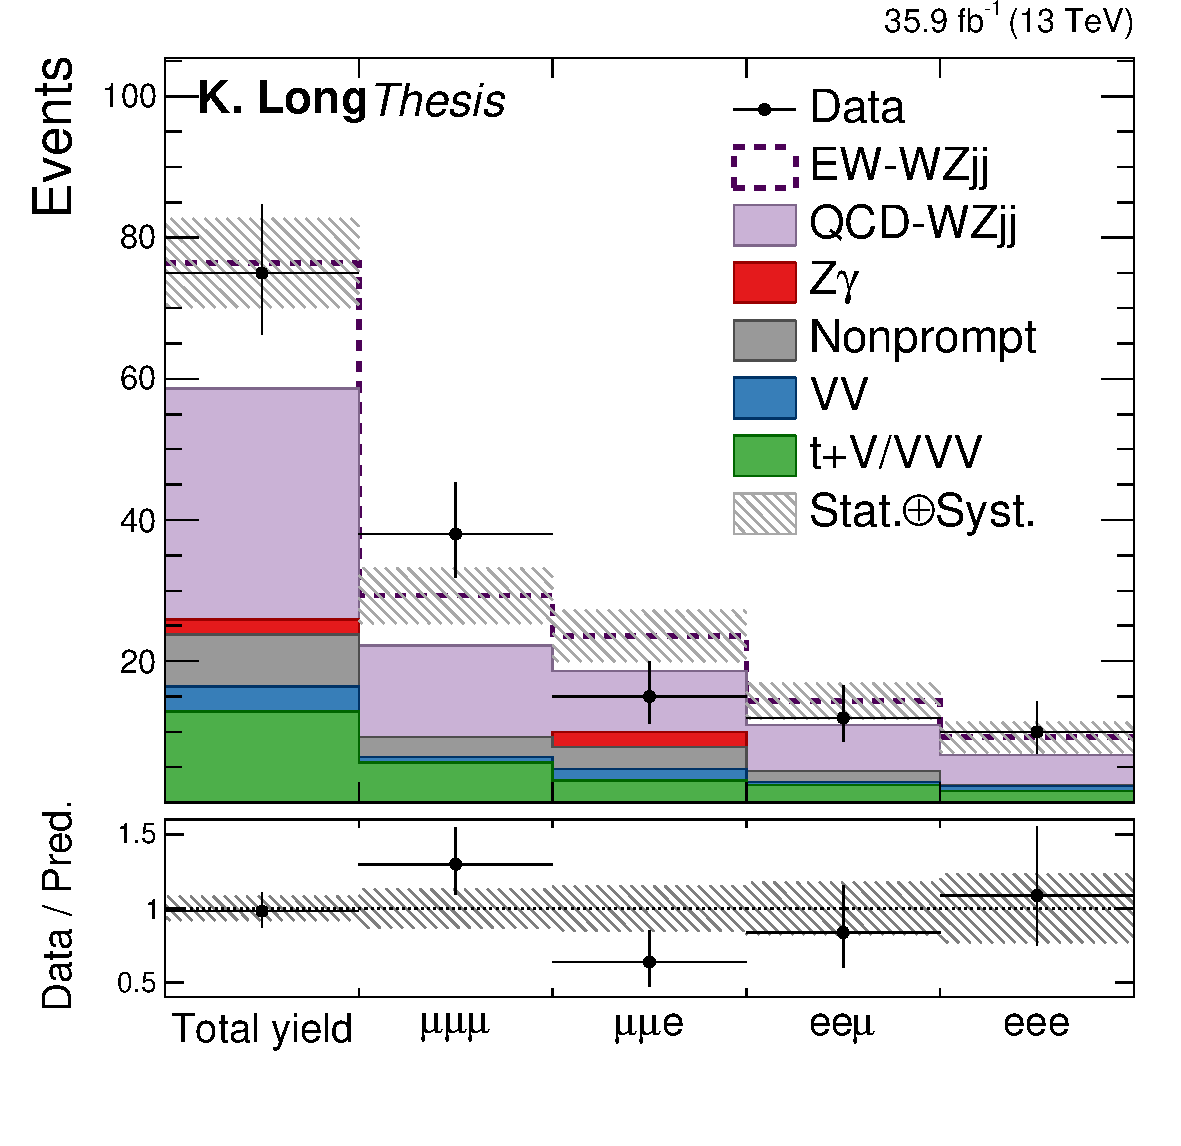
\includegraphics[width=0.7\textwidth]{figures/AnalysisResults/yieldByChannel.pdf}
  \caption{
    Post-fit event yields in the EW signal region.
          }
 \label{fig:EWSignalYields}
\end{figure}


The best fit value for the signal strength is used to obtain a cross section
in the tight fiducial region defined in Table~\ref{tab:selections}. 
The measured fiducial \WZjj cross section in this region is

\begin{equation}
  \sigma^{\mathrm{fid}}_{\mathrm{WZjj}} = 
        3.18^{+0.57}_{-0.52} \, \mathrm{(stat)} \,\, ^{+0.43}_{-0.36} \, \mathrm{(syst)}
        = 3.18^{+0.71}_{-0.63} \,\unit{fb} \,.
\end{equation}

This result can be compared to the predicted value of
$3.27 \, ^{+0.39}_{-0.32} \mathrm{(scale)} \pm 0.15\, \mathrm{(PDF)} \unit{fb}$.
The \EWWZ and \QCDWZ contributions are
calculated independently from the samples described in Section~\ref{sec:promptbackgrounds}
and their uncertainties are combined in quadrature. 
The interference term contribution in this region is less than 1\% of
the total cross section.

Results are also obtained in a looser fiducial region, defined in Table~\ref{tab:selections}
following Ref.~\cite{leshouches2017},
to simplify comparisons with theoretical calculations.
The acceptance from the loose to tight fiducial region
is $(72.4 \pm 0.8)\%$,
computed using \MG interfaced to \PYTHIA. 
The uncertainty in the acceptance is evaluated independently 
for the \EWWZ and \QCDWZ samples
from the scale
The uncertainty in the acceptance is evaluated 
by combining the scale and PDF uncertainties 
in the \EWWZ and \QCDWZ predictions in quadrature.
The scale uncertainty in the \QCDWZ contribution is the 
dominant component of the uncertainty.
The resulting \WZjj loose fiducial cross section is

\begin{equation}
  \sigma^{\mathrm{fid, loose}}_{\mathrm{WZjj}} = 
        4.39^{+0.78}_{-0.72} \, \mathrm{(stat)} \,\, ^{+0.60}_{-0.50} \, \mathrm{(syst)}
        = 4.39^{+0.98}_{-0.87} \,\unit{fb} \,,
\end{equation}

which can be compared to the predicted value of 
$4.51^{+0.59}_{-0.45} \, \mathrm{(scale)} \pm 0.18 \, \mathrm{(PDF)} \unit{fb}$.
The \EWWZ and \QCDWZ contributions 
and their uncertainties are treated independently with the same approach as described
for the tight fiducial region.

\section{Search for \EWWZ boson production}

The rate of \EWWZ production with respect to the SM prediction
is quantified by treating the \EWWZ process as signal and the \QCDWZ
process background in a binned likelihood fit to a two-dimensional
distribution of $\mjj$ and $\detajj$ as described in Section~\ref{sec:statistics}.
The observed data and the background and signal predictions,
adjusted to their best-fit values from the maximum likelihood fit,
are shown for this distribution in Fig.~\ref{fig:2DfitDistribution}.
The individual distributions of $\mjj$ and $\detajj$ are shown in
Fig.~\ref{fig:VBSPlots}.

The best-fit value for the signal strength $\mu_{\mathrm{EW}}$ is 
\begin{equation}
  \mu_{\mathrm{EW}} = 0.82^{+0.51}_{-0.43} \,,
\end{equation}
consistent with the SM expectation at LO of $\mu_{\EW,\,\mathrm{LO}} = 1$,

The significance of the signal is quantified by calculating the local $p$-value
for an upward fluctuation of the data relative to the background prediction
using a profile likelihood ratio test statistic and asymptotic formulae~\cite{Cowan:2010js}.
The observed (expected) statistical significance for \EWWZ production is 2.2 (2.5) standard deviations. 
The total uncertainty of the signal strength
measurement is dominated by the statistical uncertainty of the data.
The predicted cross section in the loose fiducial region used in the fit is 
$1.48^{+0.12}_{-0.11} \,(\mathrm{scale}) \pm 0.07 \, (\mathrm{PDF})$ fb.
The post-fit yields for the signal and background corresponding to the best-fit signal strength 
for \EWWZ production are shown in
Table~\ref{tab:VBSYields}.

\begin{figure}[htbp]
  \centering
   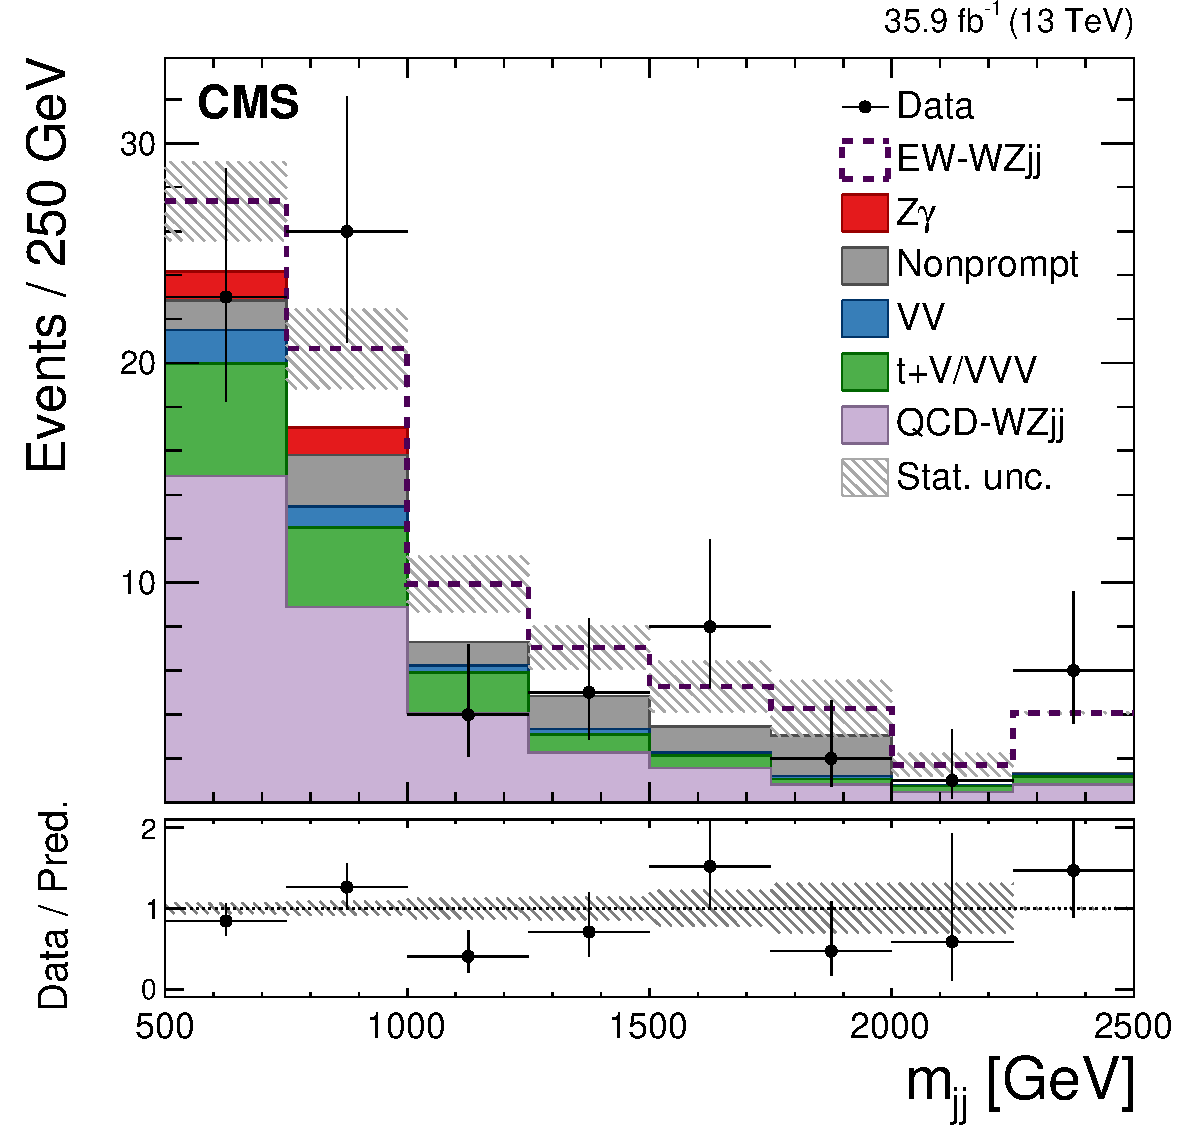
\includegraphics[width=0.49\textwidth]{figures/AnalysisResults/mjj.pdf}
   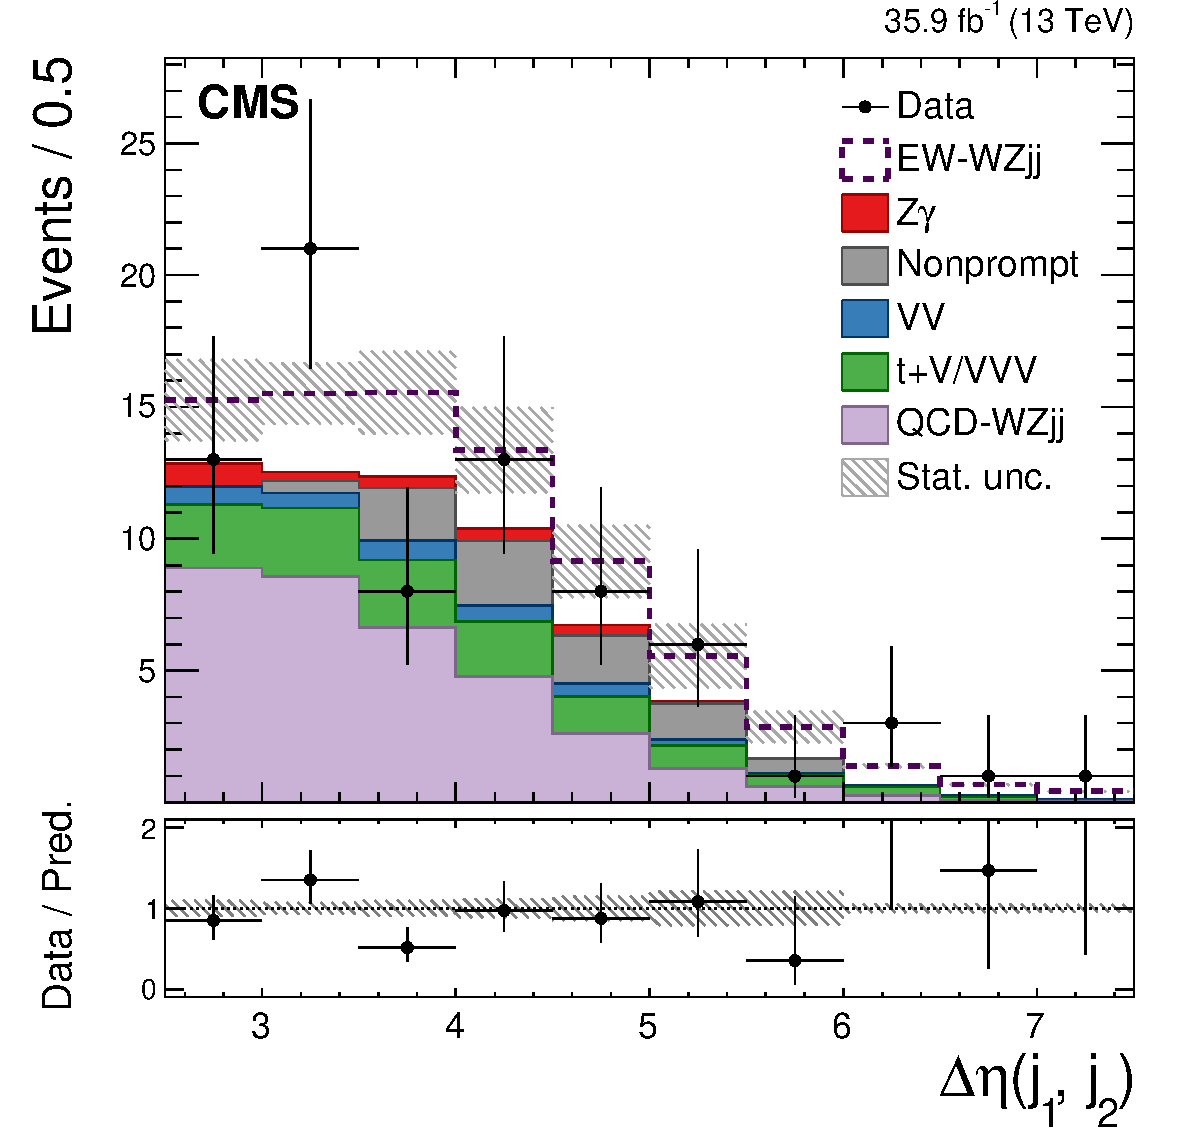
\includegraphics[width=0.49\textwidth]{figures/AnalysisResults/dEtajj.pdf}
  \caption[The observed $\mjj$ and $\left|\etajj\right|$ for events satisfying the \EW signal selection]{
    The $\mjj$ (left) and $\abs{\etajj}$ (right)
  of the two leading jets
  for events satisfying the EW signal selection.
  The last bin contains all events with $\mjj > 2500\GeV$ (left) and
  $\abs{\etajj} > 7.5$ (right).
  The dashed line shows the expected \EWWZ contribution stacked
  on top of the backgrounds that are shown as filled histograms.
  The hatched bands represent the total and relative
  statistical uncertainties on the predicted yields.
  The bottom panel shows the ratio of the number of events measured in data to the total
  number of expected events.
  The predicted yields are shown with their pre-fit normalizations.
          }
 \label{fig:VBSPlots}
\end{figure}

\begin{figure}[htbp]
  \centering
   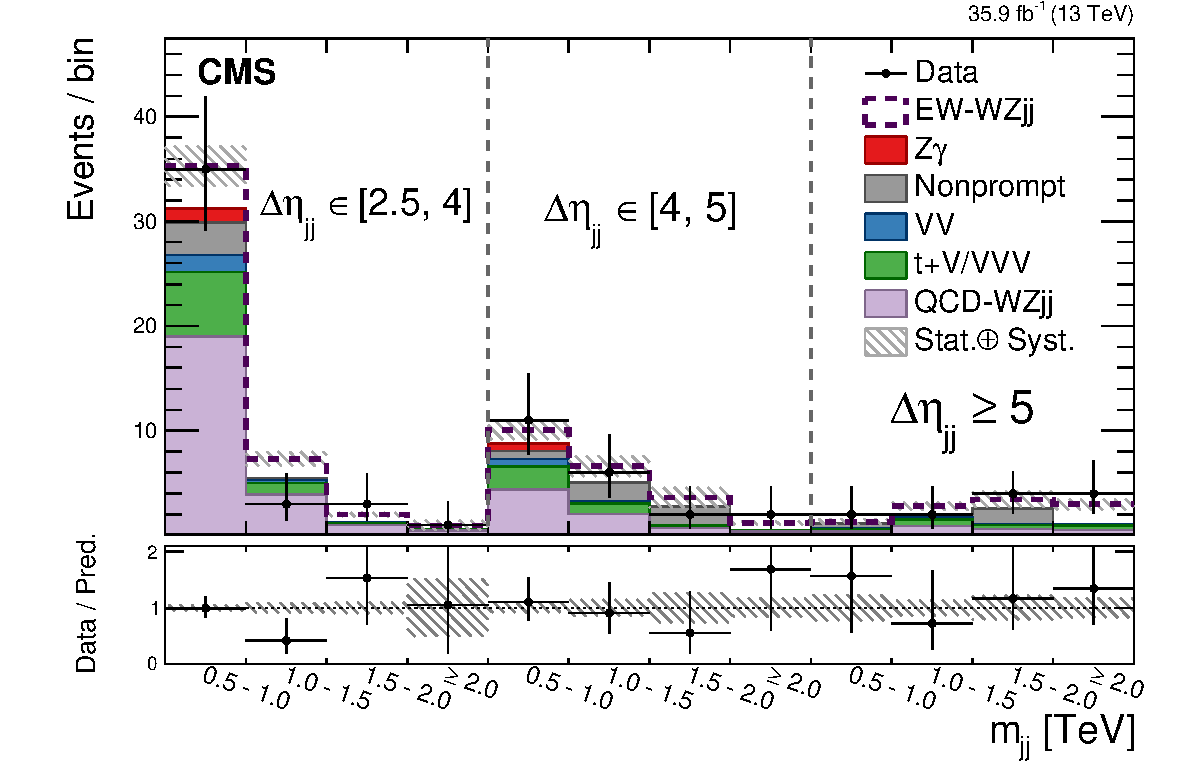
\includegraphics[width=0.7\textwidth]{figures/AnalysisResults/mjj_etajj_unrolled.pdf}
    \caption[The observed two-dimensional 2D distribution of $\mjj$ and $\left|\etajj\right|$, used for the \EW signal extraction]{
    The one-dimensional representation of the 2D distribution of
    $\mjj$ and $\abs{\etajj}$, used for the EW
    signal extraction. The x axis shows the {\mjj} distribution
    in the indicated bins, split into three bins of {\etajj }: {\etajj} $\in [2.5, 4], [4, 5], \ge 5$.
    The dashed line represents the \EWWZ contribution stacked
    on top of the backgrounds that are shown as filled histograms.
    The hatched bands represent the total and relative
    systematic uncertainties on the predicted yields.
    The bottom panel shows the ratio of the number of events measured in data to the total
    number of expected events.
    The predicted yields are shown with their best-fit normalizations.
    }
  \label{fig:2DfitDistribution}
\end{figure}

\begin{table}[htbp]
  \centering
  \caption[Post-fit event yields after the signal extraction fit to events satisfying the EW signal selection]
  {Post-fit event yields after the signal extraction fit to events satisfying the EW signal selection.
    The \EWWZ process is corrected for the observed value of $\mu_{\EW}$.}
  \begin{tabular}{lccccc}
    \hline
        Process      &      \mmm      &      \emm      &      \eem      &      \eee     &  Total yield   \\
    \hline
        \QCDWZ       & 13.5 $\pm$ 0.8 & 9.1 $\pm$ 0.5  & 6.8 $\pm$ 0.4  & 4.6 $\pm$ 0.3 & 34.1 $\pm$ 1.1 \\
       t+V/\VVV      & 5.6 $\pm$ 0.4  & 3.1 $\pm$ 0.2  & 2.5 $\pm$ 0.2  & 1.7 $\pm$ 0.1 & 12.9 $\pm$ 0.5 \\
       Nonprompt     & 5.2 $\pm$ 2.0  & 2.4 $\pm$ 0.9  & 1.5 $\pm$ 0.6  & 0.7 $\pm$ 0.3 & 9.8 $\pm$ 2.3  \\
           VV        & 0.8 $\pm$ 0.1  & 1.6 $\pm$ 0.2  & 0.4 $\pm$ 0.0  & 0.7 $\pm$ 0.1 & 3.5 $\pm$ 0.2  \\
         $\Zg$       & 0.3 $\pm$ 0.1  & 1.2 $\pm$ 0.8  & $<$0.1         & 0.6 $\pm$ 0.2 & 2.2 $\pm$ 0.8  \\
      \hline
    Pred. background & 25.5 $\pm$ 2.1 & 17.4 $\pm$ 1.5 & 11.2 $\pm$ 0.8 & 8.3 $\pm$ 0.6 & 62.4 $\pm$ 2.8 \\
     \EWWZ signal    & 6.0 $\pm$ 1.2  & 4.2 $\pm$ 0.8  & 2.9 $\pm$ 0.6  & 2.1 $\pm$ 0.4 & 15.1 $\pm$ 1.6 \\
          Data       &       38       &       15       &       12       &       10      &       75       \\
    \hline
  \end{tabular}
  \label{tab:VBSYields}
\end{table}

\subsection{Comparison with the \EWWZ measurement by the ATLAS Collaboration}
There is a small degree of tension between this result and the result
recently submitted for publication by the ATLAS 
Collaboration~\cite{Aaboud:2018ddq}, which 
reports observed signal strengths for the \EWWZ and \QCDWZ
processes of $1.77^{+0.49}_{-0.43}$ and $0.56\pm0.16$, respectively.
Because the independent results presented by the ATLAS and CMS Collaborations
are each limited by large statistical uncertainties, establishing
their mutual compatibility and compatibility with the SM will be aided by future 
experimental studies.
Because the measured signal strength is a ratio of the predicted to observed yields,
it is dependent on the MC simulation used to derive the expected yields.
While the cross sections derived from these results are not dependent on the normalization,
the fiducial regions used by the two analyses are not directly comparable.
Thus, understanding the simulations used in the two independent analyses 
in a common fiducial region will provide valuable
insight into the agreement of the two results. 
In addition, future measurements with reduced
uncertainties will definitively determine if the differences are a result
of a statistical fluctuation or if they are a consequence of different analysis
techniques or interpretations.

\begin{figure}[htbp]
  \centering
   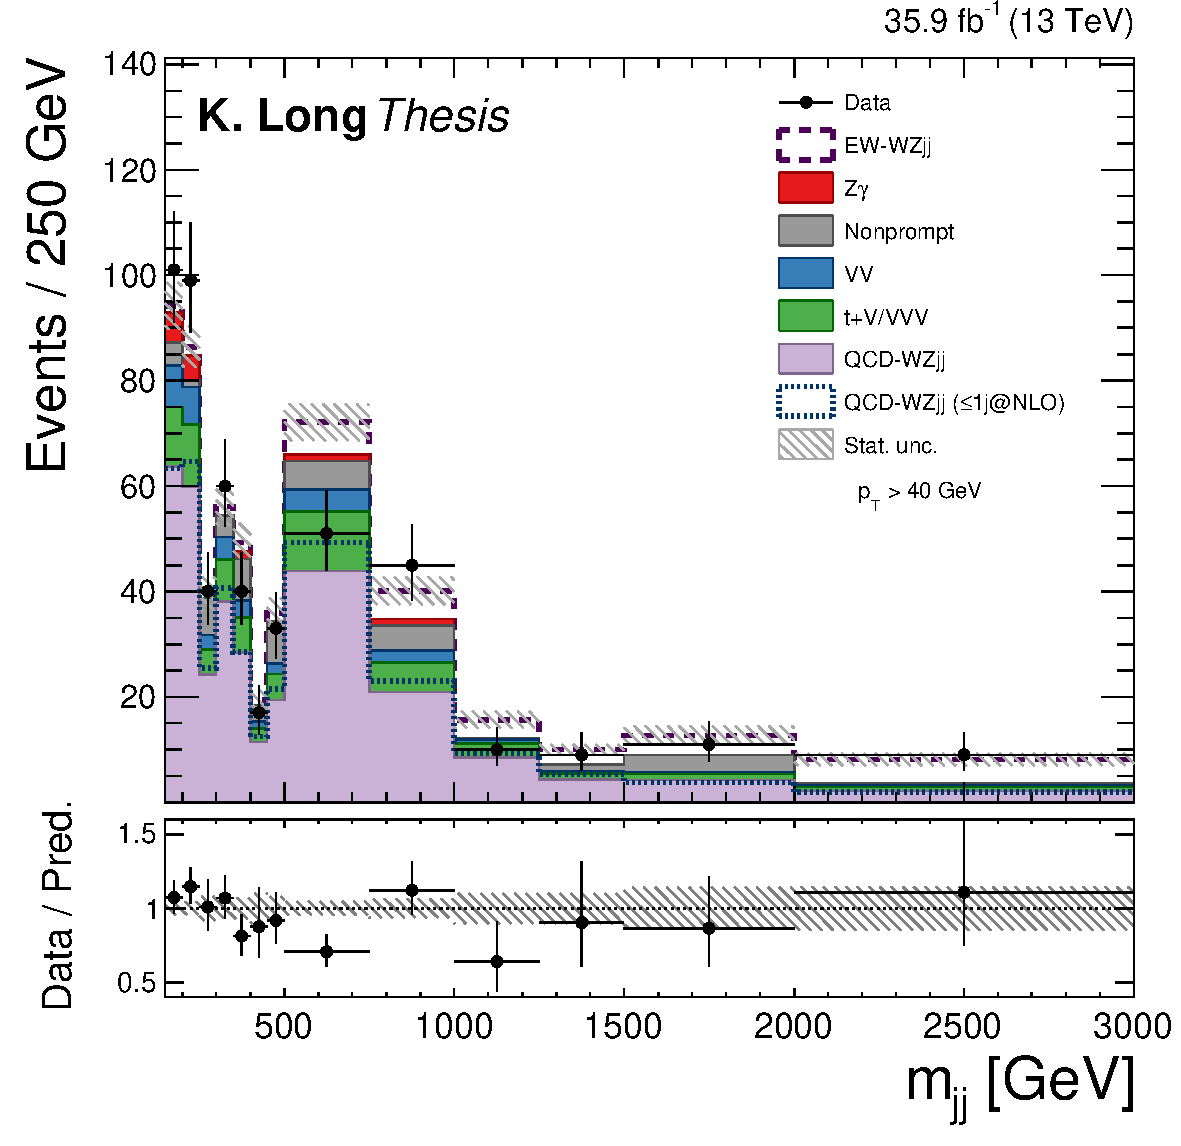
\includegraphics[width=0.49\textwidth]{figures/AnalysisResults/mjj_nMinus1_ATLASptj_Prefit.pdf}
   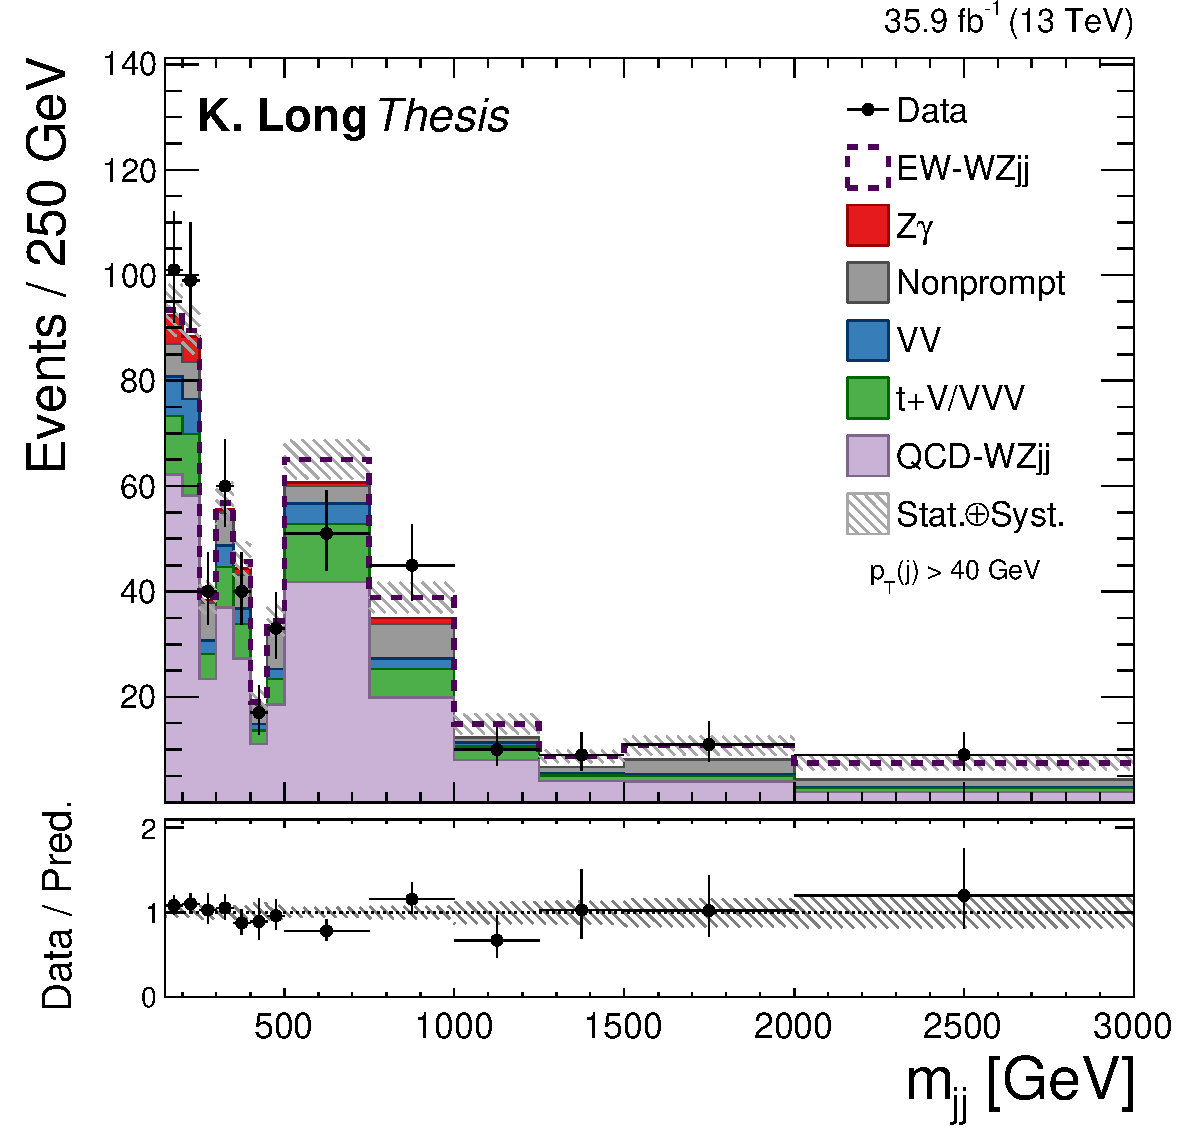
\includegraphics[width=0.49\textwidth]{figures/AnalysisResults/mjj_nMinus1_ATLASptj_Postfit.pdf}
  \caption[The $\mjj$ for events selected in a fiducial region designed to approximate the selection of the ATLAS Collaboration]{
    The $\mjj$ for events selected in a relaxed fiducial region, described in the text,
    designed to be comparable to the
    selection used by the ATLAS Collaboration in Ref.~\cite{Aaboud:2018ddq}. The distribution
    is shown with the expected normalizations input to
    the maximum likelihood fit (left) and the with the best fit normalizations
    by bin obtained from the fit (right). The data are well described by the 
    shape and normalization predicted by the MC simulations 
    of the \EWWZ (dashed purple) and \QCDWZ (filled light purple) processes
    discussed in Chapter~\ref{ch:simulation}.
        }
 \label{fig:EWWZATLASselection}
\end{figure}

The analysis presented in this thesis is designed to be sensitive
to the \EWWZ process with a minimal and explicit theoretical dependence 
on well-studied distributions.
The approach is emphasized in
Fig.~\ref{fig:EWWZATLASselection}, which shows the $\mjj$ for events in a relaxed
selection intended to mimic the fiducial region defined by the ATLAS Collaboration.
The selection is defined following Table~\ref{tab:selections}, with no condition on the
$\etajj$ or $\etas$ of the jets and with the jet transverse momentum relaxed to 40\GeV. 
To validate the results from the nominal \EWWZ signal extraction, a maximum likelihood fit
is performed to this distribution with the approach described in Chapter~\ref{ch:analysis}.
While the distribution is less sensitive to the \EWWZ process than the two-dimensional
likelihood, the central value of the \EWWZ signal strength is within 10\% of the value
presented, well within the uncertainty of the measurement. The normalization correction of the
\QCDWZ process that maximizes the likelihood is consistent with the presented result and with
unity. The distribution is well-described by the MC simulation and background estimation,
as illustrated in Fig.~\ref{fig:EWWZATLASselection}, which shows the distributions input 
to the maximum likelihood fit and the resulting best-fit distributions.
In contrast to the results of Ref.~\cite{Aaboud:2018ddq}, the distribution is
expected normalizations for the \EWWZ and \QCDWZ processes are highly consistent with the observed data.
Studies to determine if a multivariate discriminant, following the approach
of the ATLAS Collaboration, results in a different categorization of the events
as \EWWZ and \QCDWZ will be a topic of future studies.

\section{Limits on anomalous quartic gauge couplings}

Events satisfying the EW signal selection are used to constrain aQGCs in the effective field theory approach~\cite{Degrande:2012wf}.
Results are obtained following the formulation of Ref.~\cite{Eboli:2006wa} via
a maximum likelihood fit to the $\mt$ as described in Section~\ref{sec:aqgcProcedure}.
The $\mt$ for events satisfying the
EW signal selection is shown in Fig~\ref{fig:aQGCDistribution}. The predictions of several
indicative aQGC operators and coefficients are also shown.

The one-dimensional 95\% confidence level (CL) limits are extracted 
using the CL$\mathrm{_s}$ criterion~\cite{Junk:1999kv,CLS2,Cowan:2010js}, with all parameters
except for the coefficient being probed set to zero.
The SM prediction, including the \EWWZ process, is treated as the null hypothesis.
No deviation from the SM prediction is observed, 
and the resulting observed and expected limits are summarized in Table~\ref{tab:1Dlimits}. 

\begin{figure}[htbp]
  \centering
    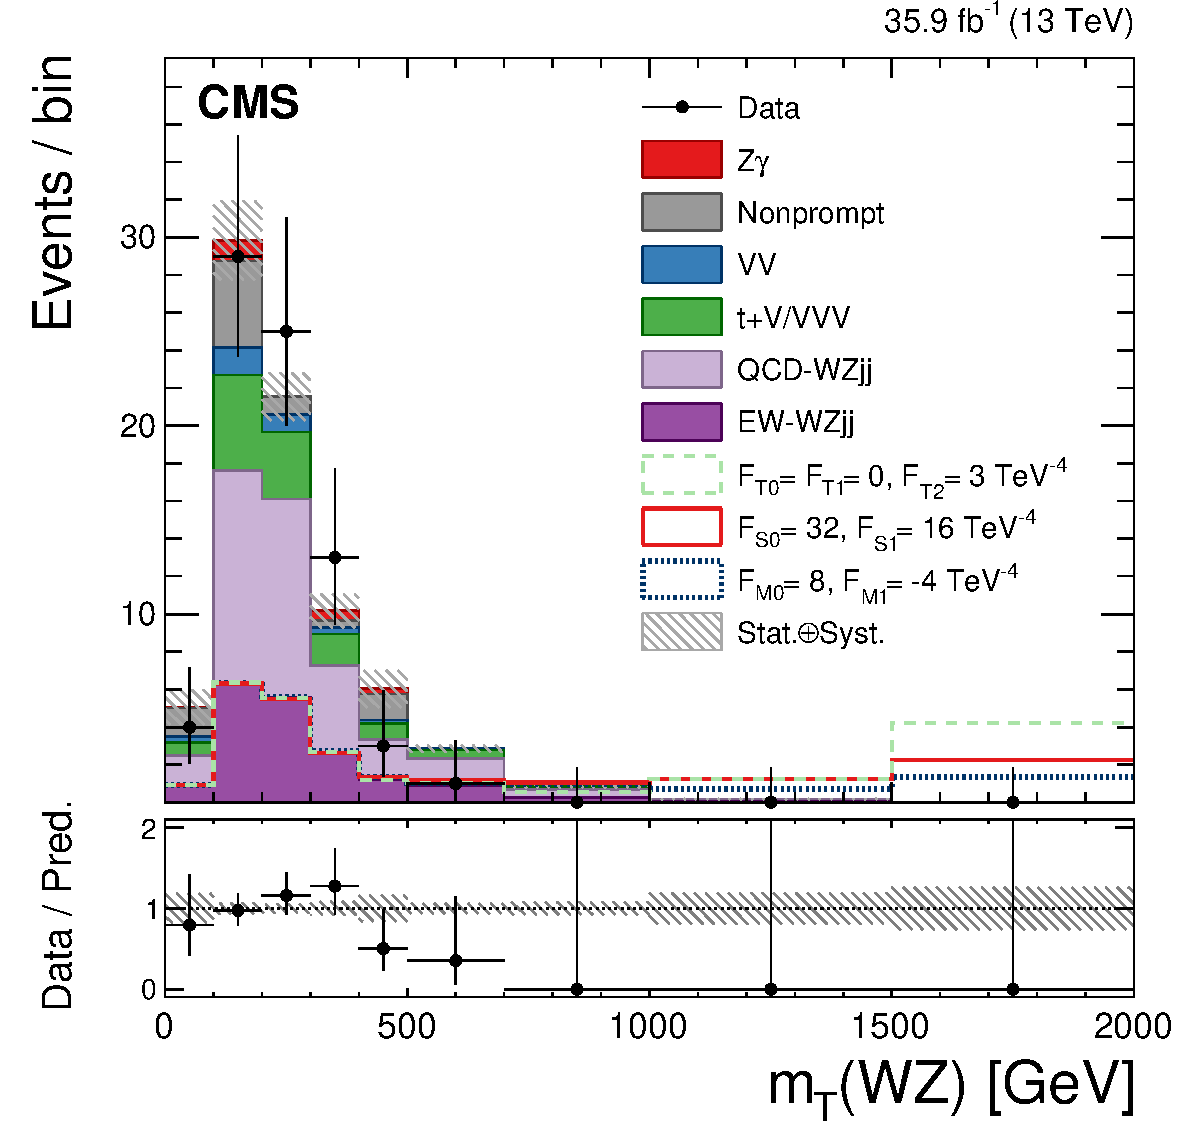
\includegraphics[width=0.7\textwidth]{figures/AnalysisResults/MTWZ_aQGC.pdf}
  \caption[The observed $\mt$ for events satisfying the EW signal selection]{
      The $\mt$ for events satisfying the EW signal selection,
      used to place constraints on the anomalous coupling parameters.
      The dashed lines show predictions for several aQGC parameters values that modify the \EWWZ process.
      The last bin contains all events with $\mt > 2000\GeV$.
      The hatched bands represent the total and relative 
      systematic uncertainties on the predicted yields.
      The bottom panel shows the ratio of the number of events measured in data to the total 
      number of expected events. 
      The predicted yields are shown with their best-fit normalizations from the background-only fit.
      }
 \label{fig:aQGCDistribution}
\end{figure}

\begin{table} [htbp]
\centering
  \caption[Observed and expected 95\% CL limits for each operator coefficient while all other parameters are set to zero]
  {Observed and expected 95\% CL limits for each operator coefficient while all other parameters are set to zero.}
\begin{tabular}{ccc}
\hline 
  Parameters & Expected limit ($\TeV^{-4}$) & Observed limit ($\TeV^{-4}$) \\ 
\hline
f$_{\text{M0}}/\Lambda^4$ & $[-11.2, 11.6]$ & $[-9.15, 9.15]$ \\  
f$_{\text{M1}}/\Lambda^4$ & $[-10.9, 11.6]$ & $[-9.15, 9.45]$ \\  
f$_{\text{S0}}/\Lambda^4$ & $[-32.5, 34.5]$ & $[-26.5, 27.5]$ \\  
f$_{\text{S1}}/\Lambda^4$ & $[-50.2, 53.2]$ & $[-41.2, 42.8]$ \\
f$_{\text{T0}}/\Lambda^4$ & $[-0.87, 0.89]$ & $[-0.75, 0.81]$ \\ 
f$_{\text{T1}}/\Lambda^4$ & $[-0.56, 0.60]$ & $[-0.49, 0.55]$ \\  
f$_{\text{T2}}/\Lambda^4$ & $[-1.78, 2.00]$ & $[-1.49, 1.85]$ \\ 
\hline 
\end{tabular} 
\label{tab:1Dlimits}
\end{table}

Constraints are also placed on aQGC parameters using a two-dimensional scan,
where two parameters are probed in the fit with all others set to zero.
The resulting 2D 95\% CL intervals for these parameters are shown in Fig.~\ref{fig:2Dlimits}.\\

\begin{figure}[htbp]
  \centering
   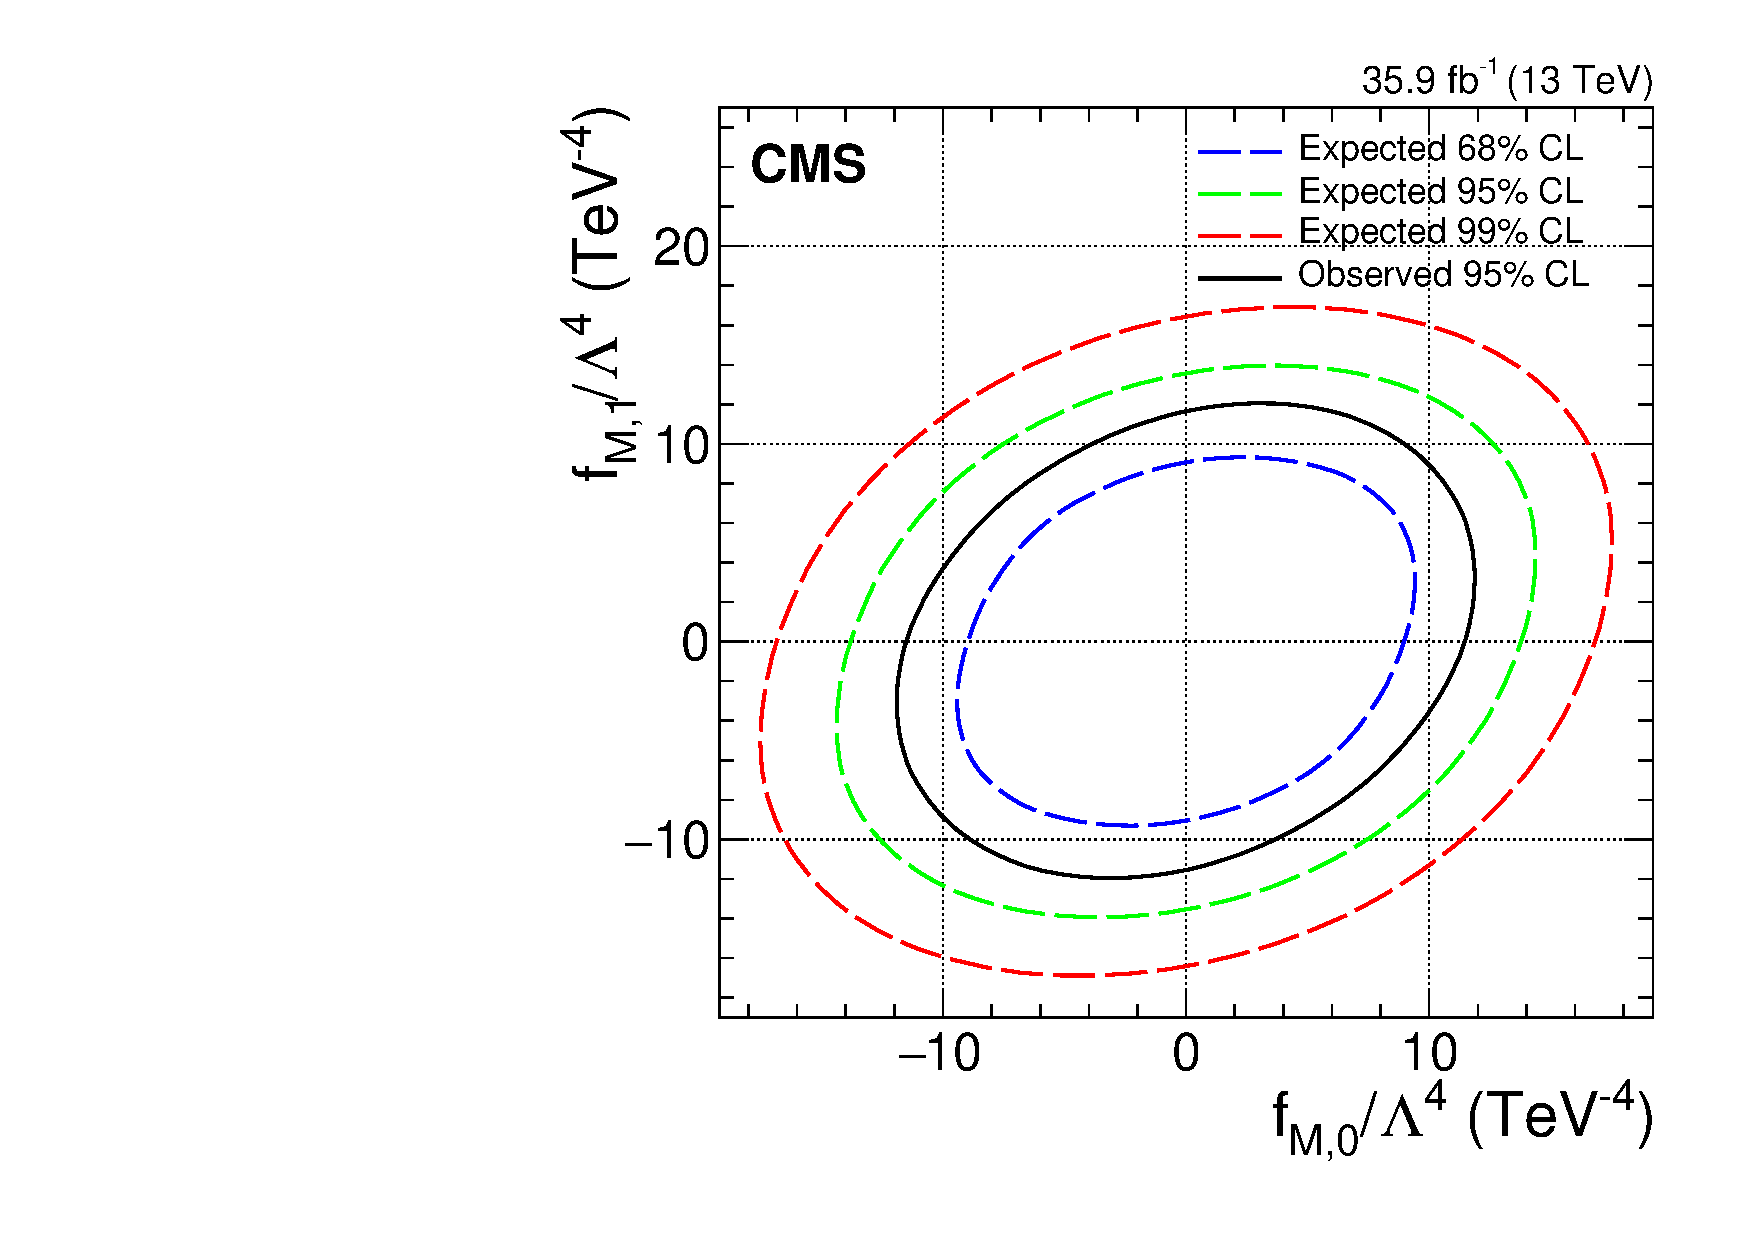
\includegraphics[width=0.49\textwidth]{figures/AnalysisResults/fm0_fm1_2dlimit_deltaNLL_WZ_aQGC.pdf}
   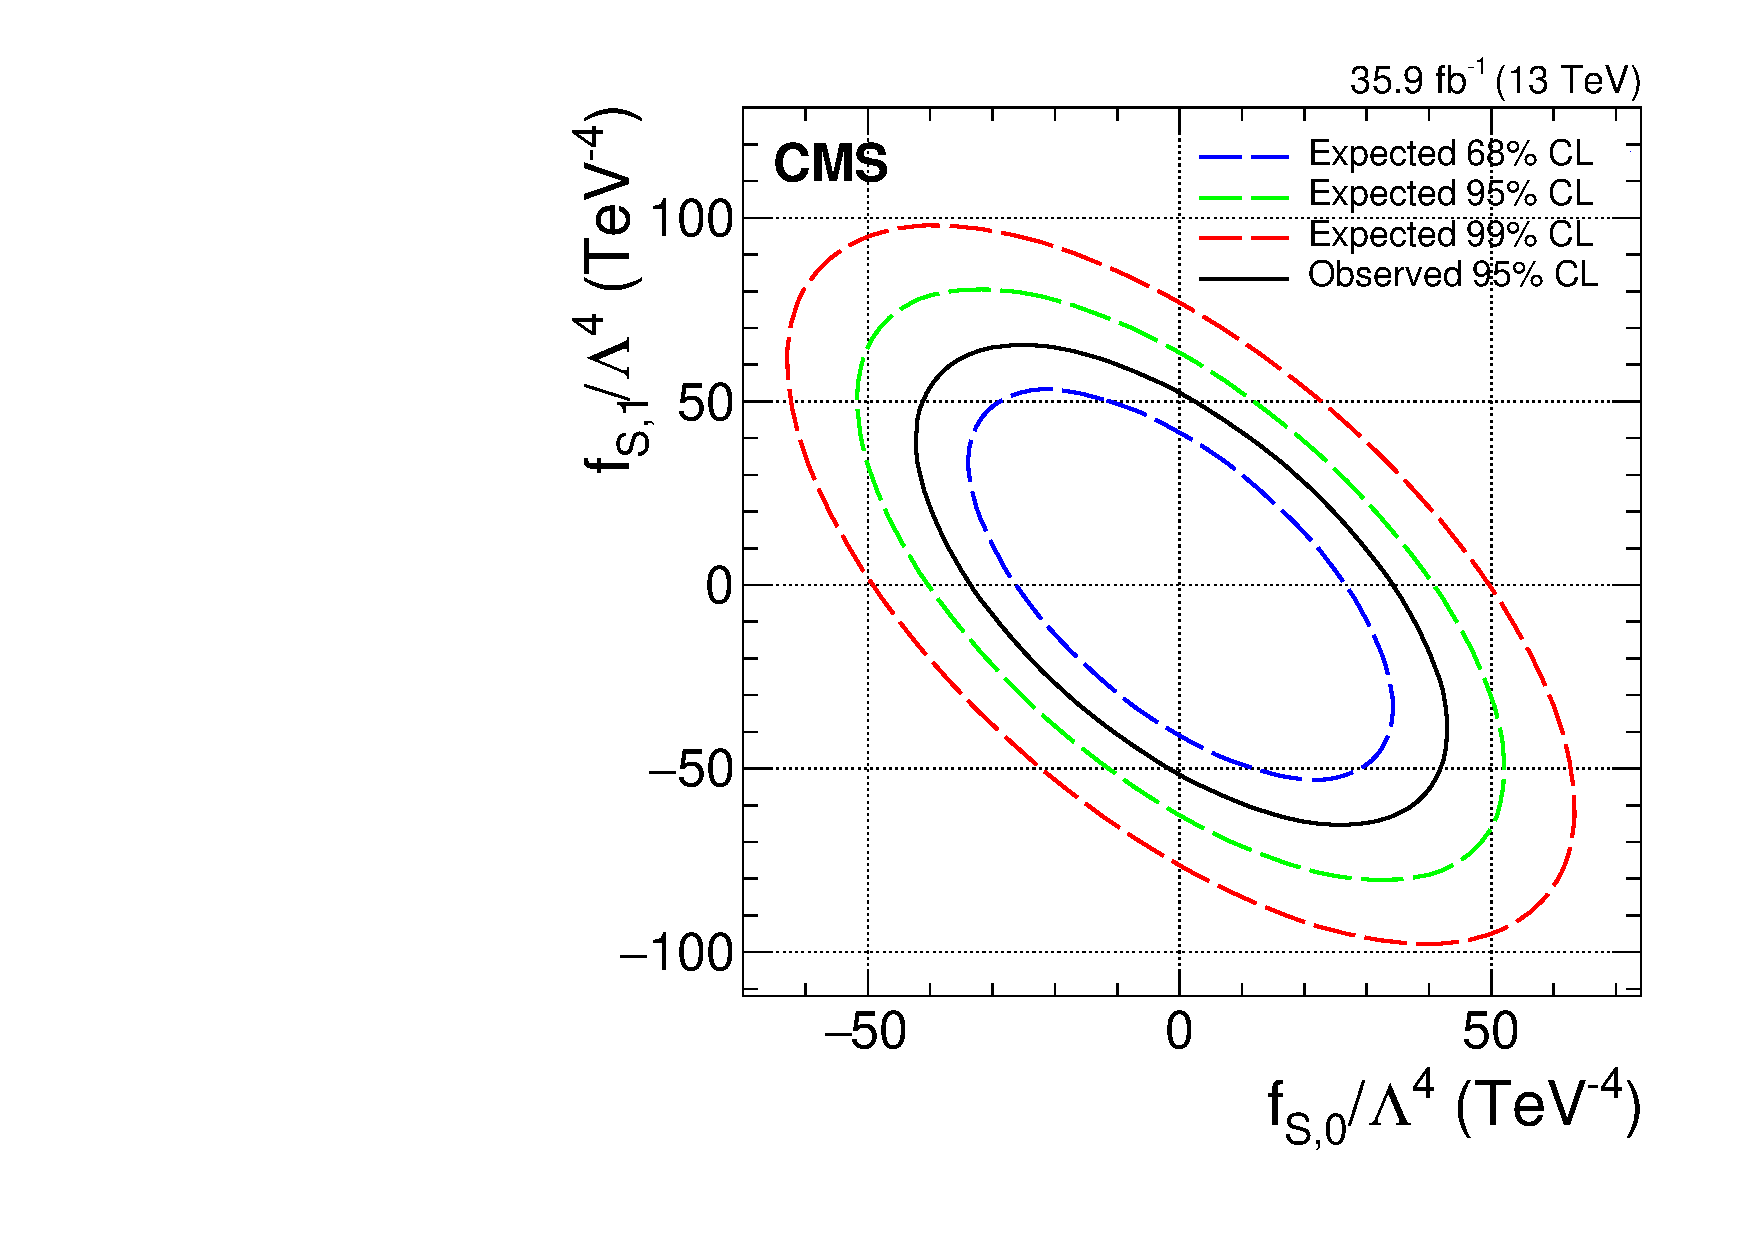
\includegraphics[width=0.49\textwidth]{figures/AnalysisResults/fs0_fs1_2dlimit_deltaNLL_WZ_aQGC.pdf}
  \caption[Two-dimensional observed and expected 95\% CL intervals on selected aQGC parameters]
  {Two-dimensional observed 95\% CL intervals (solid contour) and expected
68, 95, and 99\% CL intervals (dashed contour) on the selected aQGC parameters.
The values of coefficients 
outside of contours are excluded at the corresponding CL.
 }
 \label{fig:2Dlimits}
\end{figure}

Constraints on aQGCs in terms of dimension-eight effective field theory operators
have also been obtained by analyses of \EW VV events in other production and decay channels.
The results presented
here are competitive with constraints from analyses exploiting leptonic decays,
as shown in Fig.~\ref{fig:aQGCCompareFS} and \ref{fig:aQGCCompareFT} for the 
T0, T1, T2, S0, and S1 operators. 
The most stringent results using leptonic decays are obtained by the CMS Collaboration
using the \EW $\Wpm\Wpm$\cite{Sirunyan:2017ret} 
channel at 13\TeV. 
A preliminary study using VV events where one boson decays hadronically and one leptonically
has recently been performed by the CMS Collaboration~\cite{CMS-PAS-SMP-18-008}, which 
significantly extends the constraints on 
operators sensitive to charged interactions.

\begin{figure}[htbp]
  \centering
   \includegraphics[width=0.9\textwidth]{figures/AnalysisResults/aQGC_ft.pdf}
  \caption[Comparison of experimental constraints on the T0, T1, and T2 EFT operators]
  {
    Comparison of 95\% CL intervals on the T0, T1, and T2 dimension-eight EFT operators 
    obtained by the ATLAS and CMS Collaborations. 
 }
 \label{fig:aQGCCompareFT}
\end{figure}

\begin{figure}[htbp]
  \centering
   \includegraphics[width=0.9\textwidth]{figures/AnalysisResults/aQGC_fs.pdf}
  \caption[Comparison of experimental constraints on the S0 and S1 dimension-eight EFT operators]
  {
    Comparison of 95\% CL intervals on the S0 and S1 dimension-eight EFT operators 
    obtained by the ATLAS and CMS Collaborations. 
 }
 \label{fig:aQGCCompareFS}
\end{figure}

\section{Limits on charged Higgs boson production}

The observed event yields by channel, and expected yields adjusted to the
best-fit values obtained from a maximum likelihood fit in the charged Higgs
boson selection described in Section~\ref{sec:eventselection} 
are shown in Fig.~\ref{fig:higgsSignalYields}.

\begin{figure}[htbp]
  \centering
   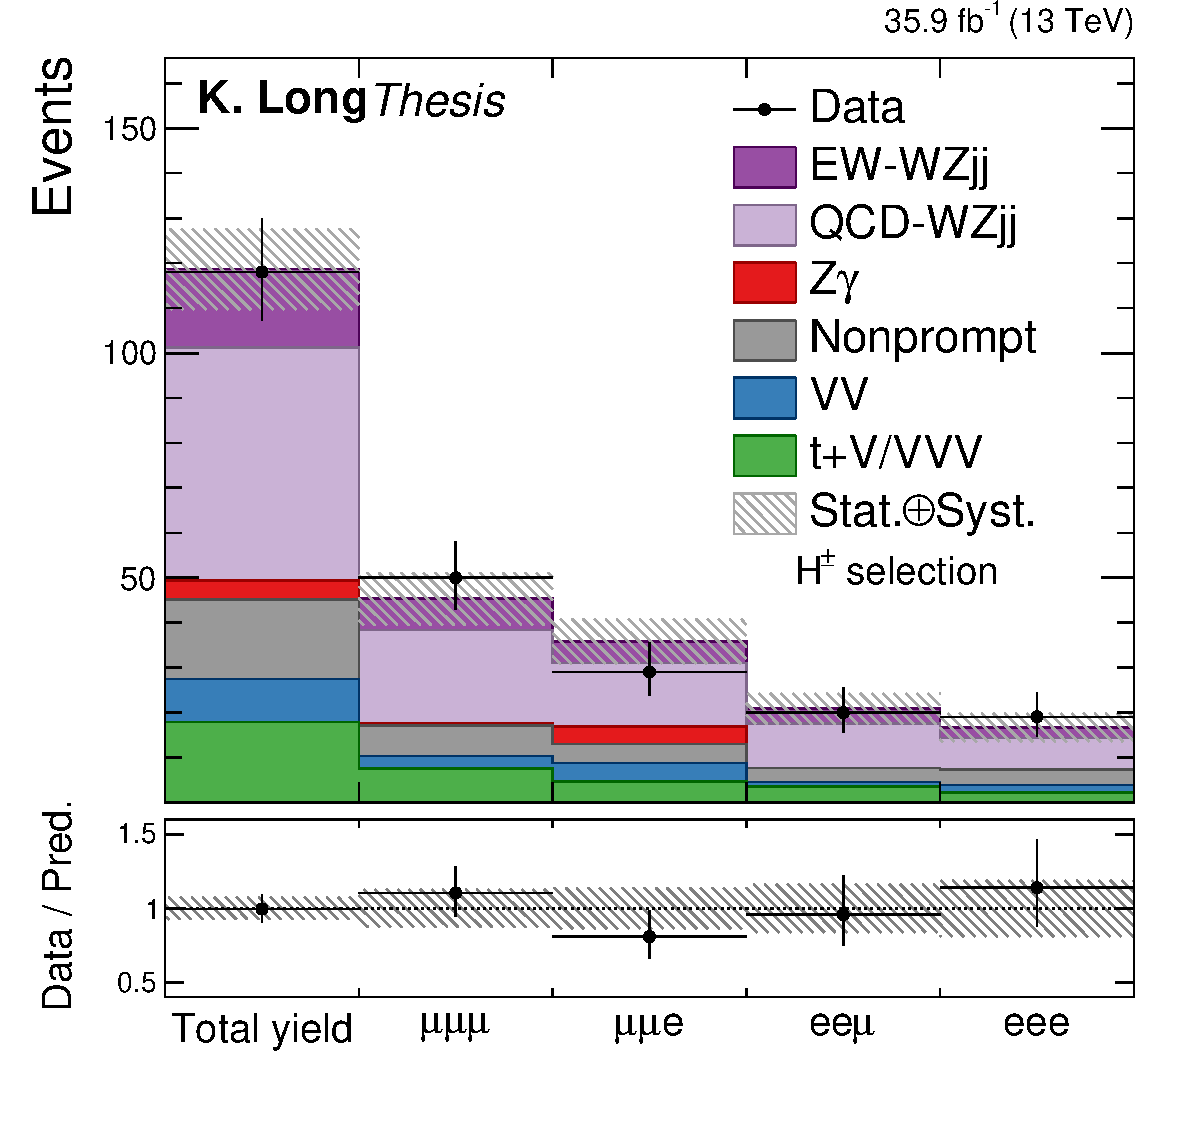
\includegraphics[width=0.6\textwidth]{figures/AnalysisResults/yieldByChannel_Higgs.pdf}
  \caption{
    Post-fit event yields in the charged Higgs boson search region.
          }
 \label{fig:higgsSignalYields}
\end{figure}

Constraints on the production of charged Higgs bosons are derived via
a maximum likelihood fit of the expected yields to the data in 
a control region of events with $\mjj > 100\GeV$ 
outside the signal selection and the $\mt$ for events the charged Higgs boson
selection. The $\mt$ distribution for the observed data and expected background,
as well as illustrative predictions for charged Higgs boson production in the 
Georgi-Machacek model are shown in Fig.~\ref{fig:higgsmt}.
No deviation from the SM prediction is observed, 
and the resulting observed and expected limits are summarized in 
Fig.~\ref{fig:higgsLimits}.
Limits are derived on the production cross section in a largely model-independent way,
assuming a narrow-width charged Higgs boson produced via vector boson fusion,
and in the Georgi-Machecek model. Results in the Georgi-Machacek model are 
presented in terms of the parameter $s_{\rm H}$ and the mass of the charged 
Higgs boson. These limits are directly comparable to other searches for charged
and doubly-charged Higgs bosons in this model.

\begin{figure}[htbp]
  \centering
    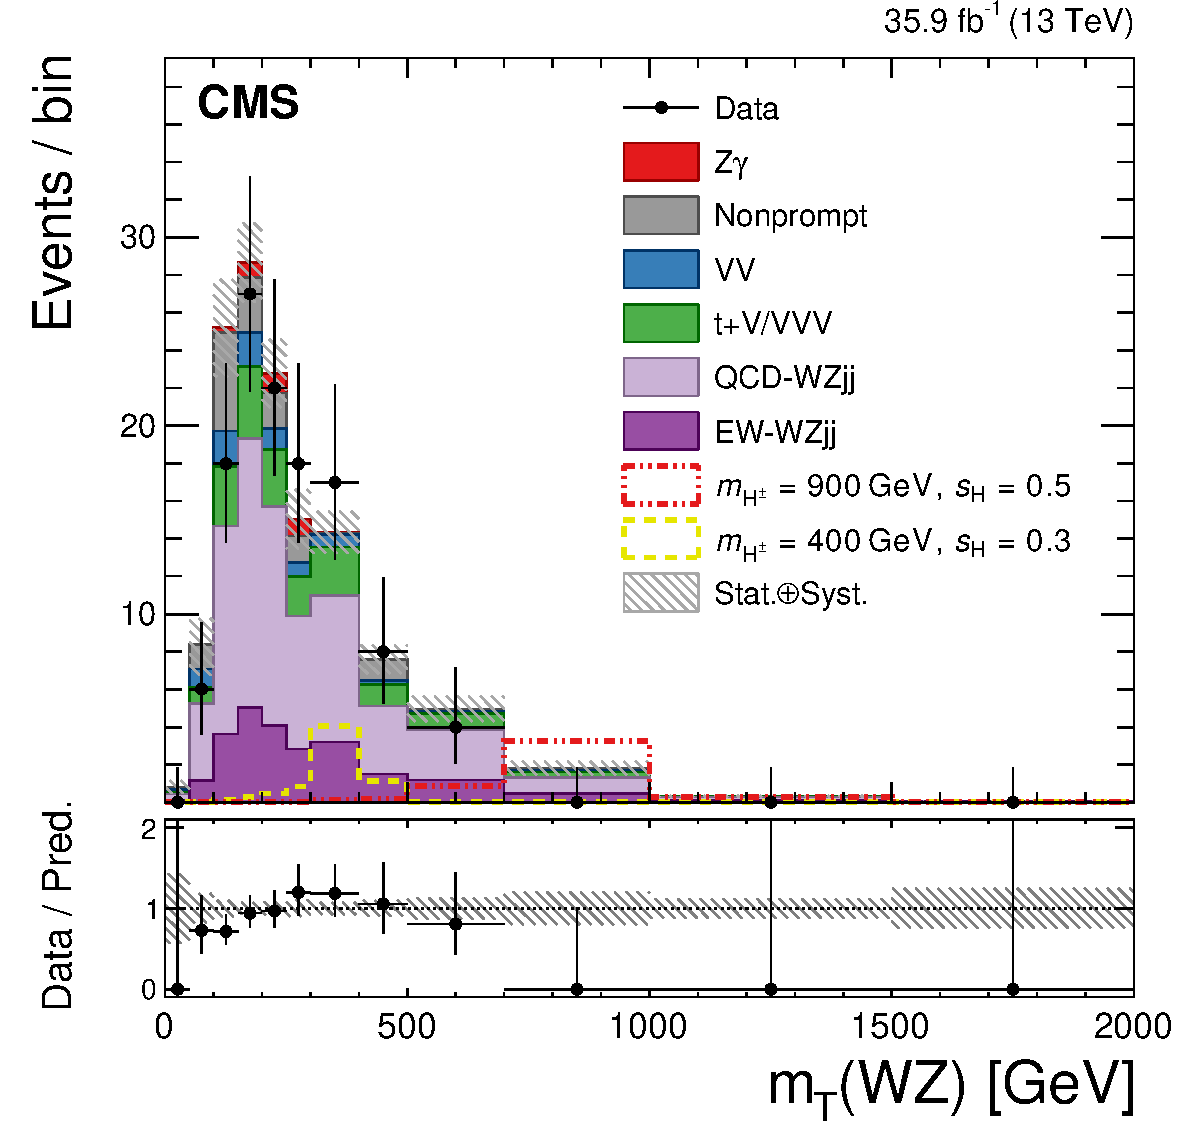
\includegraphics[width=0.6\textwidth]{figures/AnalysisResults/MTWZ_Higgs.pdf}
  \caption[The observed $\mt$ for events satisfying the Higgs boson selection]{
      The observed $\mt$ for events satisfying the Higgs boson selection,
      used to place constraints on the production of charged Higgs bosons.
      The last bin contains all events with $\mt > 2000\GeV$.
      The dashed lines show predictions from the Georgi-Machechek model with
      $m(\PHpm) = 500 \,(900)\GeV$ and $s_{\PH} = 0.3 \,(0.5)$.
      The bottom panel shows the ratio of the number of events measured in data to the total 
      number of expected events. The hatched bands represent the total and relative 
      systematic uncertainties on the predicted background yields.
      The predicted yields are shown with their best-fit normalizations from the background-only fit.
      }
 \label{fig:higgsmt}
\end{figure}

\begin{figure}[htbp]
\begin{center}
  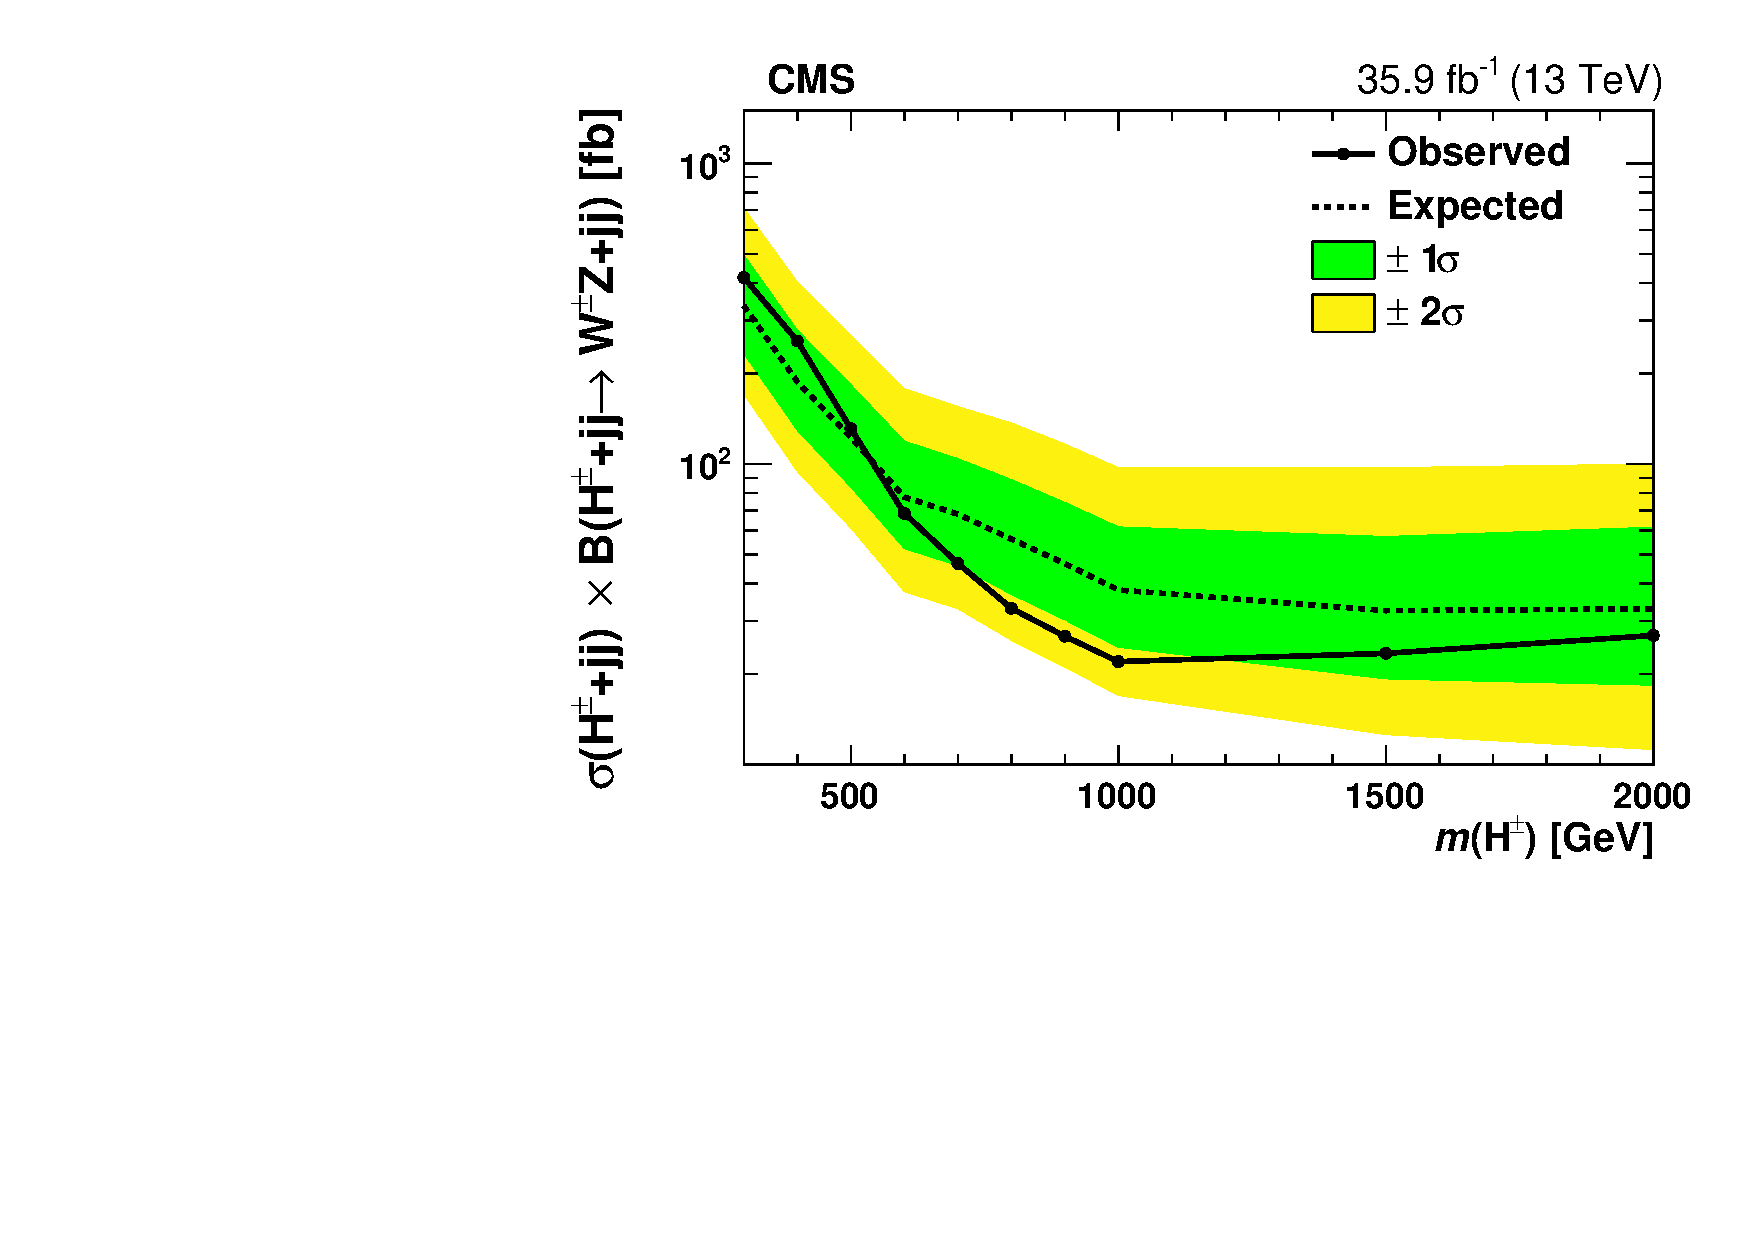
\includegraphics[width=0.6\textwidth]{figures/AnalysisResults/limits_Ind.pdf}
  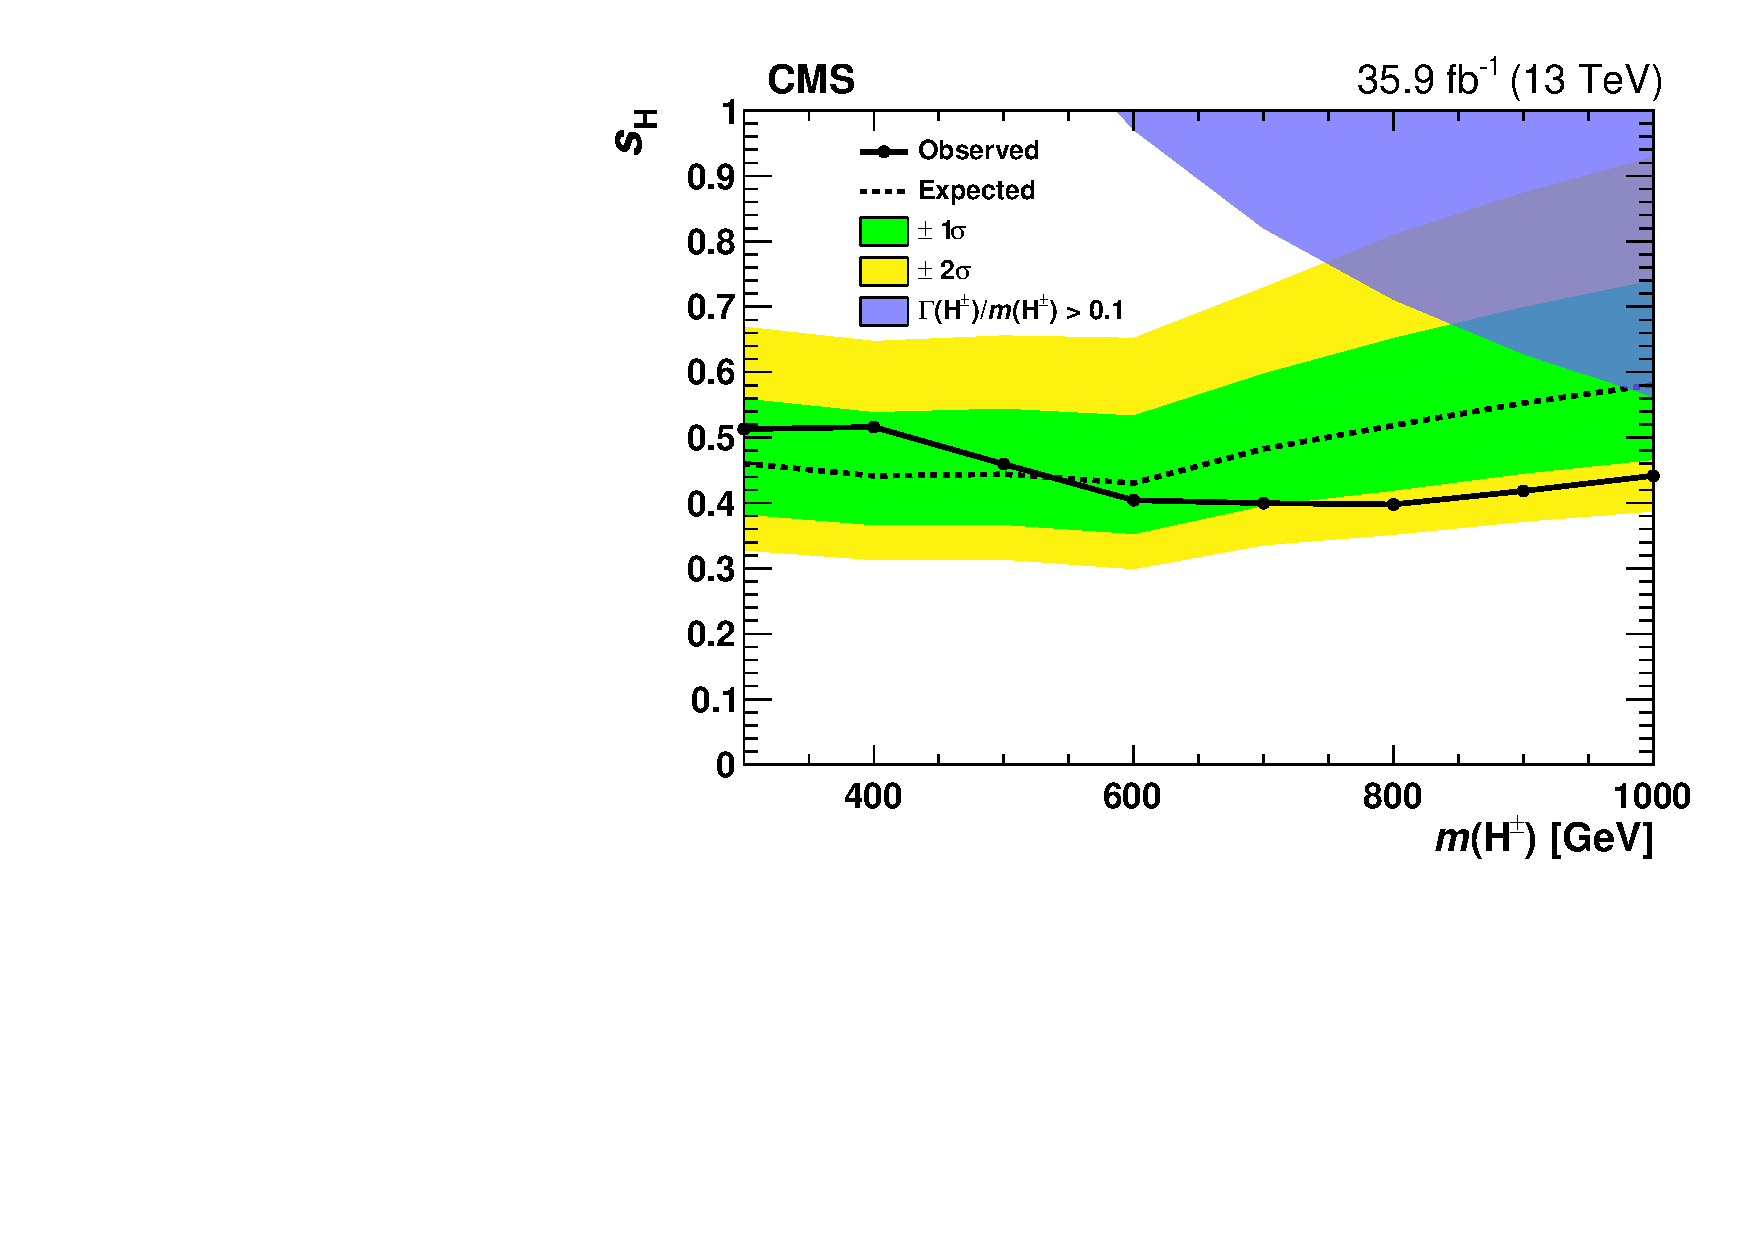
\includegraphics[width=0.6\textwidth]{figures/AnalysisResults/limits_GM.pdf}
  \caption[Expected and observed upper limits at 95\% CL on charged Higgs boson production]{
  Expected (dashed lines)
  and observed (solid lines) upper limits at 95\% CL for the model independent 
  $\sigma(\mathrm{H}^{\pm}) \times \mathcal{B}(H^+\rightarrow \WZ)$ 
  as a function of $m(\mathrm{H}^\pm)$ (left) and $s_{\PH}$ in the Georgi--Machacek model (right).
  The blue shaded area covers the theoretically not allowed parameter space~\cite{Zaro:2002500}.
}
\label{fig:higgsLimits}
\end{center}
\end{figure}

